\documentclass{beamer}
\usepackage{amsmath, amssymb}
\usepackage{physics}
\usepackage{subfig}
\usepackage{hyperref}

\usepackage[utf8]{inputenc}
\usetheme{default}

\title{Usage of JEWEL generator}
\author{Jinghong Yang}

\begin{document}

\begin{frame}
\titlepage
\end{frame}

\begin{frame}
\frametitle{Table of Contents}
\tableofcontents
\end{frame}

\section{Installation}
\begin{frame}
 \frametitle{Installing prerequisites}

 \begin{figure}[h]
  \centering
  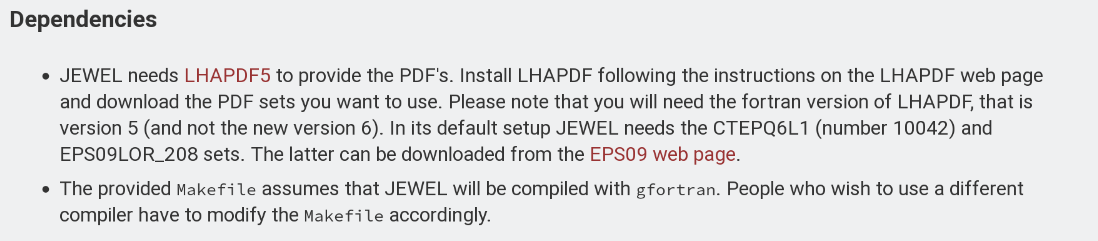
\includegraphics[width=0.9\linewidth]{dependencies.png}
 \end{figure}

 \begin{itemize}
  \item Download LHAPDF5
 \end{itemize}


\end{frame}

\section{Data generation}

\section{Data processing using RIVET}

\section{Generate gluon and quark jets}

\section{Troubleshooting}

\end{document}


